
\chapter{全日本学生飛行ロボットコンテスト}
\section{飛行ロボットコンテストについて}
本研究室では,一貫したマルチコプター製作の中間目標として全日本学生室内飛行ロボットコンテストマルチコプター部門に出場した.
全日本学生室内飛行ロボットコンテストは,室内で飛行する航空機型ロボットによる競技で,マルチコプター部門は,「ドローン」と呼ばれることが多い,複数の回転翼をもつ機体(マルチコプター)で出場します.
同部門のミッションは,ヘリポートから飛行を開始し,ミッションエリアにて各ミッションを完了したのち,ヘリポートに帰還する.


\begin{figure}[htbp]
  \begin{center}
    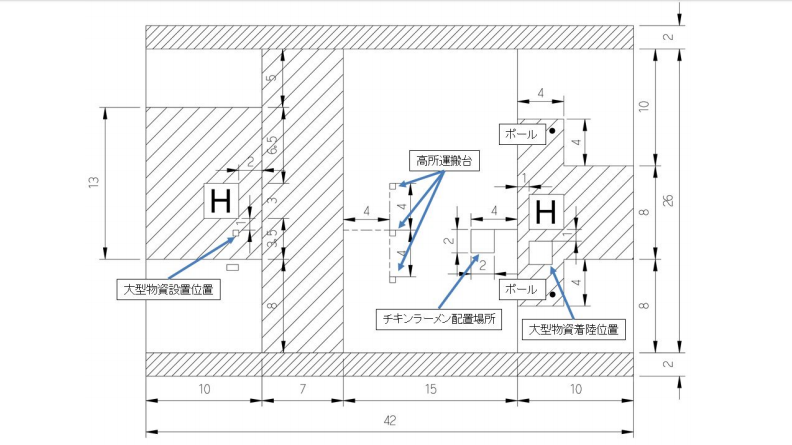
\includegraphics[width=150mm]{img/17.png}
    \end{center}
  \caption{飛行協議エリア}
 \label{fig:robot}

\end{figure}\begin{figure}[htbp]
  \begin{center}
    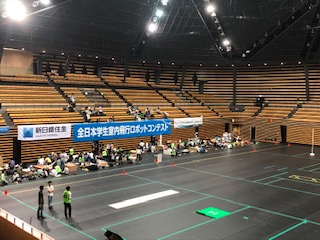
\includegraphics[width=120mm]{img/20.JPG}
    \end{center}
  \caption{大会会場}
 \label{fig:robot}
\end{figure}

\section{大会結果}
今年の予選のミッションは,離陸して高所から物資(チキンラーメン)を正解の高所運搬台に運び,運んだチキンラーメンの数で点数を競い,この,ミッションをクリアすれば「8の字飛行」にチャレンジし,速度や性能を競う.
決勝では,大型の物資運搬にチャレンジし,離着陸エリアからぬいぐるみを結び付けて離陸して,着陸位置にぬいぐるみを静止させ.
接続を保ったままヘリポートに機体を着陸させる.予選と決勝を通じて全てのチャレンジに成功し満点を獲得した.
また,これまでマルチコプター部門には,2回エントリーして2回とも書類審査を通過できず3度目の挑戦で優勝をすることができた.

\begin{figure}[htbp]
  \begin{center}
    \includegraphics[width=120mm]{img/2.JPG}
    \end{center}
  \caption{大会出場機体}
 \label{fig:robot}
\end{figure}